\documentclass[10pt]{beamer}
\usepackage[english]{babel}
\usepackage[utf8]{inputenc}
\usepackage[T1]{fontenc}
\usepackage{helvet}
\usepackage{lipsum}  
\usepackage{graphicx, subfigure}


%-------------------------------------------------------
% INFORMATION IN THE TITLE PAGE
%-------------------------------------------------------

\newcommand{\cstitle}{\textbf{Deep Learning and Transformers in MHC-peptide Binding and Presentation Towards Personalized Vaccines in Cancer Immunology: A Brief Review}
\subtitle[]{Tésis de doctorado}}
\newcommand{\cscourseCode}{PACBB Doctoral Consortium}
\newcommand{\csauthor}{MSc. Vicente Machaca Arceda}
\institute[UNSA]{Universidad La Salle}
\newcommand{\csemail}{vmachaca@utec.edu.pe}
\newcommand{\instituteabr}{UTEC}
\newcommand{\nameUp}{}
\date{2023}
\title[\cscourseCode]{\cstitle}
\author{\csauthor}
%%%%%%%%%%%%%%%%%

%-------------------------------------------------------
% CHOOSE THE THEME
%-------------------------------------------------------
\def\mycmd{0} % UNSA
\def\mycmd{1} % SALLE
%\def\mycmd{2} % UTEC
%-------------------------------------------------------

\if\mycmd0
\usepackage{csformat}
\newcommand{\chref}[3][blue]{\href{#2}{\color{#1}{#3}}}%

\fi

\if\mycmd1
\usetheme[]{Feather}
\newcommand{\chref}[2]{	\href{#1}{{\usebeamercolor[bg]{Feather}#2}} }
\fi

\if\mycmd2
\usetheme{UTEC2020}	
\newcommand{\chref}[3][blue]{\href{#2}{\color{#1}{#3}}}%
\fi

\newcommand{\1}{
	\setbeamertemplate{background}{
		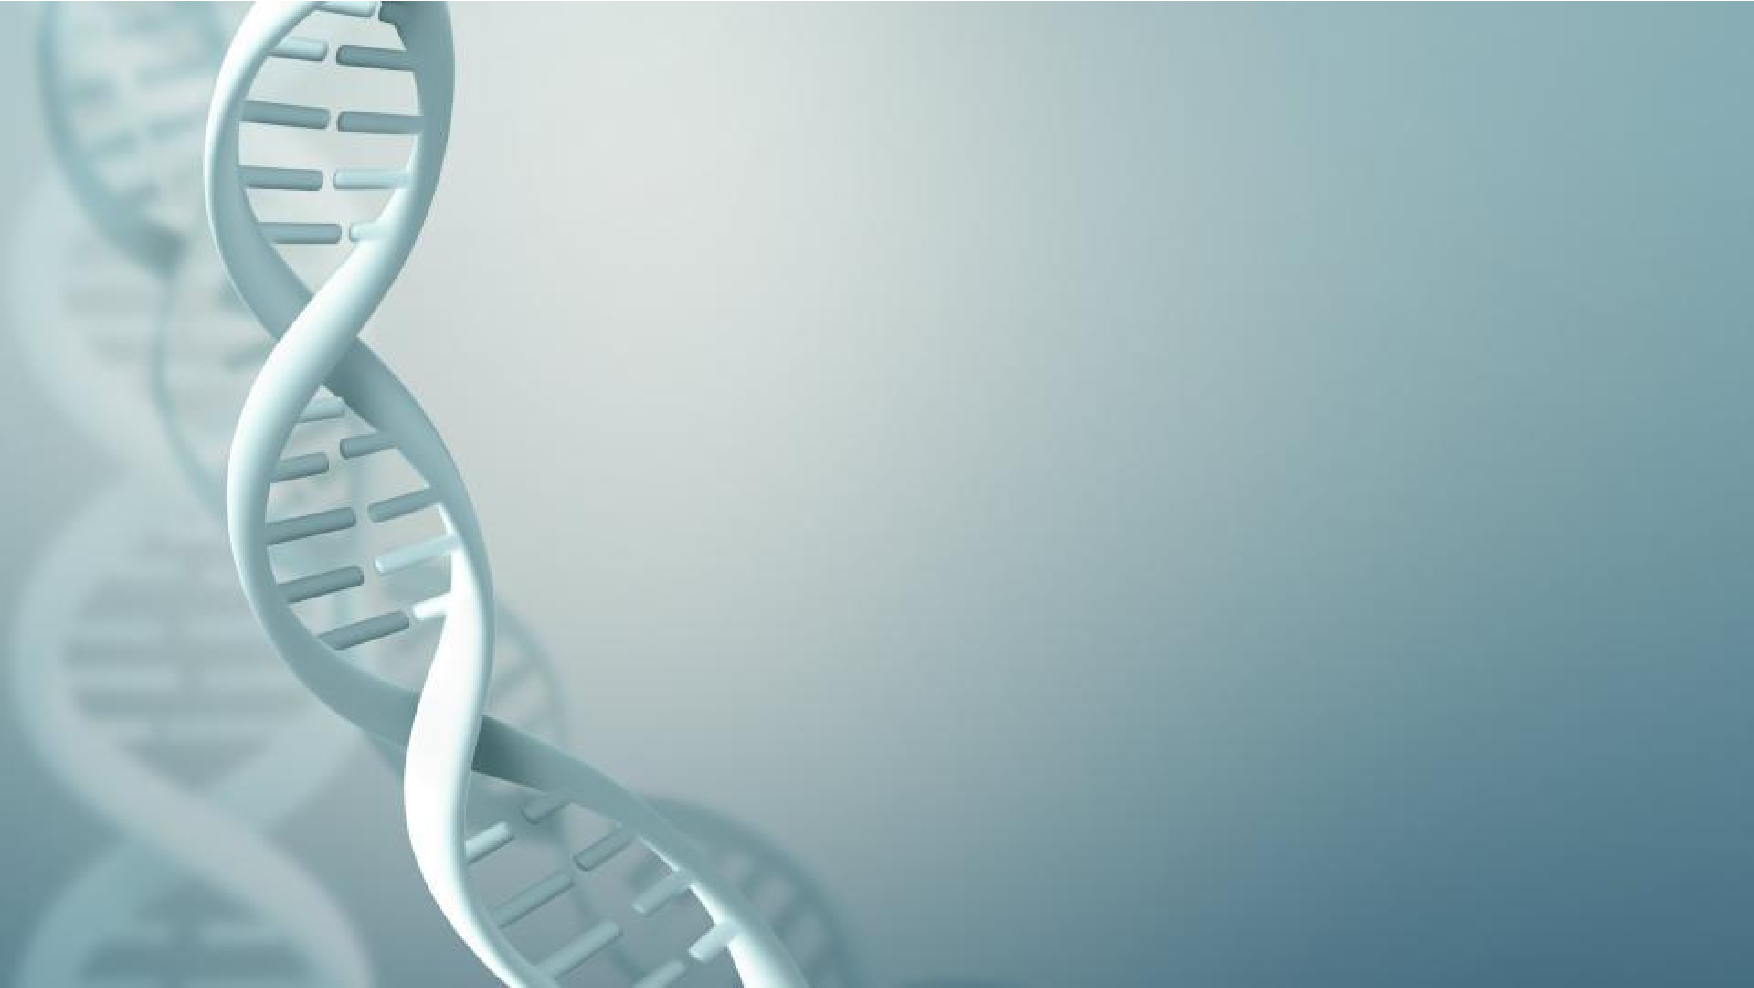
\includegraphics[width=\paperwidth,height=\paperheight]{img/1}
		\tikz[overlay] \fill[fill opacity=0.75,fill=white] (0,0) rectangle (-\paperwidth,\paperheight);
	}
}



%-------------------------------------------------------
% THE BODY OF THE PRESENTATION
%-------------------------------------------------------

\begin{document}
	
	
	\AtBeginSubsection[]
	{
		\begin{frame}
			\frametitle{Content}
			\tableofcontents[currentsubsection]
		\end{frame}
	}
	
	
	%-------------------------------------------------------
	% THE TITLEPAGE
	%-------------------------------------------------------
	
	\if\mycmd0
	\maketitle
	\fi
	
	\if\mycmd1 % MY THEME
	\1{
		\begin{frame}[plain,noframenumbering] 
			\titlepage 
	\end{frame}}
	\fi
	
	\if\mycmd2
	\begin{frame}
		\titlepage
	\end{frame}
	\fi
	%-------------------------------------------------------
	%-------------------------------------------------------


%-------------------------------------------------------
%-------------------------------------------------------
\begin{frame}{Content}
	\tableofcontents
\end{frame}
%-------------------------------------------------------
%-------------------------------------------------------


%%%%%%%%%%%%%%%%%%%%%%%%%%%%%%%%%%%%%%%%%%%%%%%%%%%%%%%%%%%%%%%%%%%%%%%%%%%%%%%%%%%%%%%%%%%%%%%%%%%%%%%%%%%%%%%%
%%%%%%%%%%%%%%%%%%%%%%%%%%%%%%%%%%%%%%%%%%%%%%%%%%%%%%%%%%%%%%%%%%%%%%%%%%%%%%%%%%%%%%%%%%%%%%%%%%%%%%%%%%%%%%%%
%%%%%%%%%%%%%%%%%%%%%%%%%%%%%%%%%%%%%%%%%%%%%%%%%%%%%%%%%%%%%%%%%%%%%%%%%%%%%%%%%%%%%%%%%%%%%%%%%%%%%%%%%%%%%%%%
\section{Introduction}
%%%%%%%%%%%%%%%%%%%%%%%%%%%%%%%%%%%%%%%%%%%%%%%%%%%%%%%%%%%%%%%%%%%%%%%%%%%%%%%%%%%%%%%%%%%%%%%%%%%%%%%%%%%%%%%%
%%%%%%%%%%%%%%%%%%%%%%%%%%%%%%%%%%%%%%%%%%%%%%%%%%%%%%%%%%%%%%%%%%%%%%%%%%%%%%%%%%%%%%%%%%%%%%%%%%%%%%%%%%%%%%%%
%%%%%%%%%%%%%%%%%%%%%%%%%%%%%%%%%%%%%%%%%%%%%%%%%%%%%%%%%%%%%%%%%%%%%%%%%%%%%%%%%%%%%%%%%%%%%%%%%%%%%%%%%%%%%%%%


%%%%%%%%%%%%%%%%%%%%%%%%%%%%%%%%%%%%%%%%%%%%%%%%%%%%%%%%%%%%%%%%%%%%%%%%%%%%%%%%%%%%%%%%%%%%%%%%%%%%%%%%%%%%%%%%
%%%%%%%%%%%%%%%%%%%%%%%%%%%%%%%%%%%%%%%%%%%%%%%%%%%%%%%%%%%%%%%%%%%%%%%%%%%%%%%%%%%%%%%%%%%%%%%%%%%%%%%%%%%%%%%%
%%%%%%%%%%%%%%%%%%%%%%%%%%%%%%%%%%%%%%%%%%%%%%%%%%%%%%%%%%%%%%%%%%%%%%%%%%%%%%%%%%%%%%%%%%%%%%%%%%%%%%%%%%%%%%%%
\subsection{Immunotherapy to Treat Cancer}
%%%%%%%%%%%%%%%%%%%%%%%%%%%%%%%%%%%%%%%%%%%%%%%%%%%%%%%%%%%%%%%%%%%%%%%%%%%%%%%%%%%%%%%%%%%%%%%%%%%%%%%%%%%%%%%%
%%%%%%%%%%%%%%%%%%%%%%%%%%%%%%%%%%%%%%%%%%%%%%%%%%%%%%%%%%%%%%%%%%%%%%%%%%%%%%%%%%%%%%%%%%%%%%%%%%%%%%%%%%%%%%%%
%%%%%%%%%%%%%%%%%%%%%%%%%%%%%%%%%%%%%%%%%%%%%%%%%%%%%%%%%%%%%%%%%%%%%%%%%%%%%%%%%%%%%%%%%%%%%%%%%%%%%%%%%%%%%%%%

%-------------------------------------------------------
%-------------------------------------------------------
\begin{frame}{Immunotherapy to Treat Cancer}{}		
	Immunotherapy is a type of cancer treatment that helps your immune system fight cancer \cite{inmunoterapy2022}.
	
	\begin{figure}
		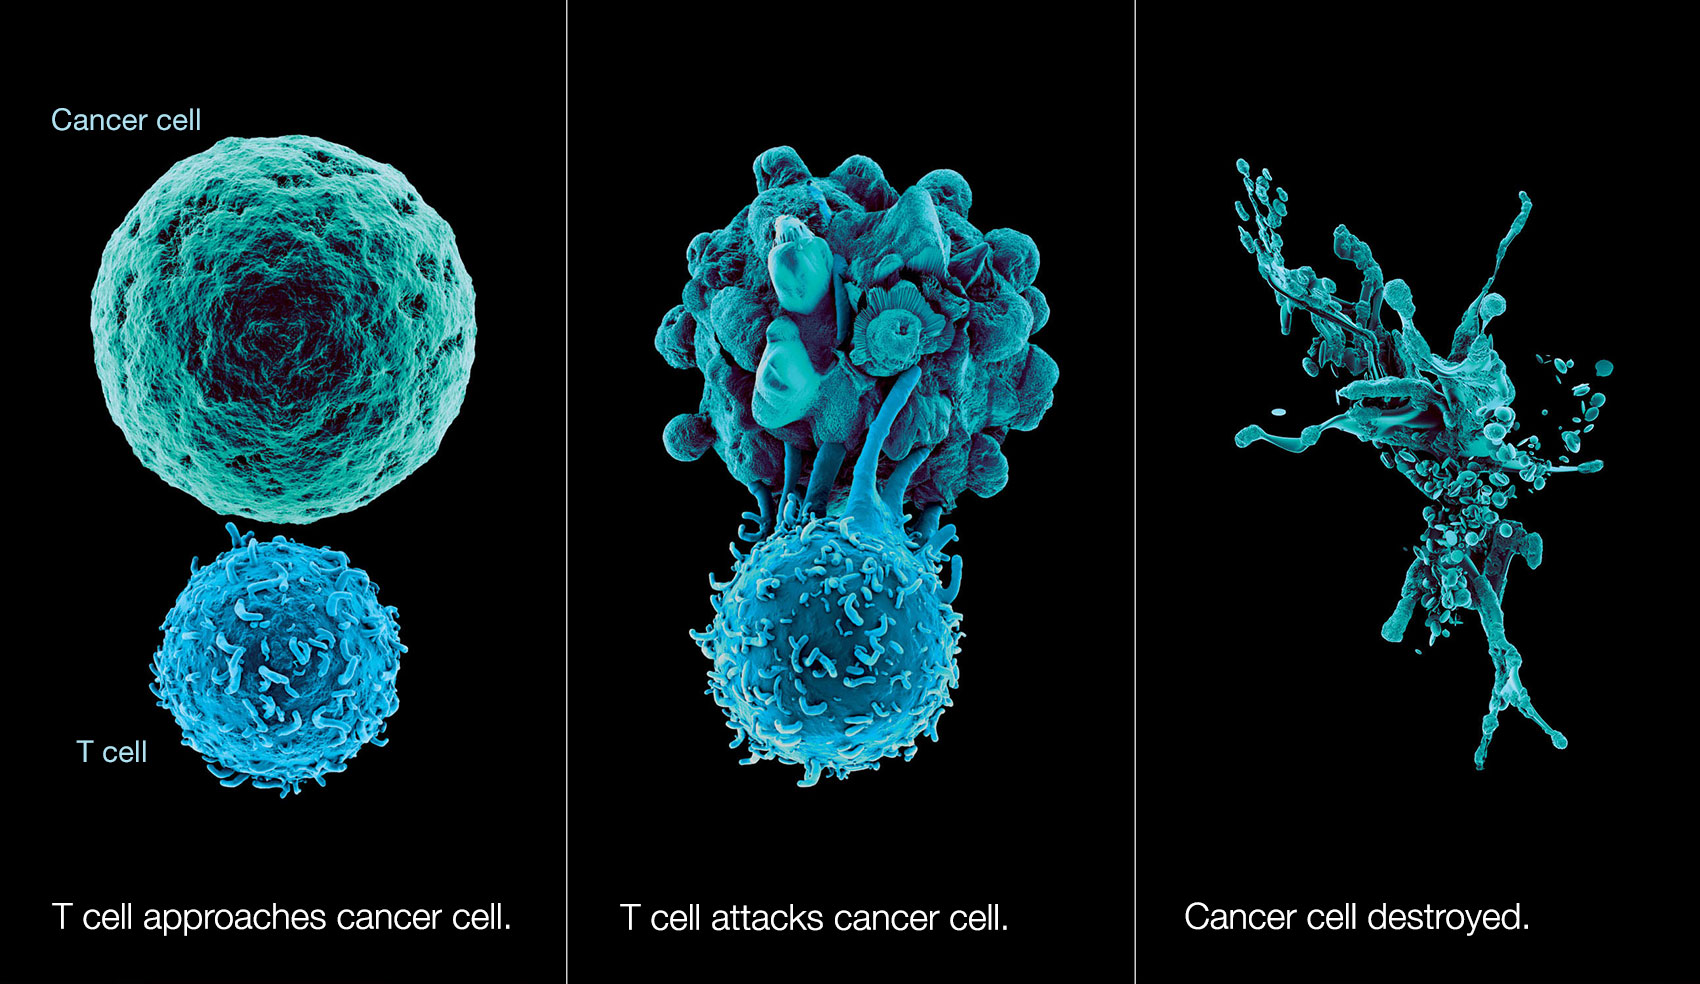
\includegraphics[width=0.85\textwidth]{img/neoantigen/tcell}
		\caption{Example of how a T cell attack a cancer cell \cite{nortshore2022}.}
	\end{figure}		
\end{frame}
%-------------------------------------------------------
%-------------------------------------------------------

%-------------------------------------------------------
%-------------------------------------------------------
\begin{frame}{Immunotherapy to Treat Cancer}{Neoantigen}		
	\begin{block}{Neoantigen}
		A new protein that forms on cancer cells when certain mutations occur in tumor DNA. Neoantigens used in vaccines and other types of immunotherapy are being studied in the treatment of many types of cancer \cite{NCIdictionary2022, borden2022cancer}.
	\end{block} 
	\begin{block}{}
		Currently, there is a lot of methods to detect neoantigens; however, only a small number of them manage to stimulate the immune system \cite{chen2021challenges, hao2021improvement}.
	\end{block}
\end{frame}
%-------------------------------------------------------
%-------------------------------------------------------


%-------------------------------------------------------
%-------------------------------------------------------
\begin{frame}{Immunotherapy for Cancer}{Personalized Vaccines}	
	\begin{figure}
		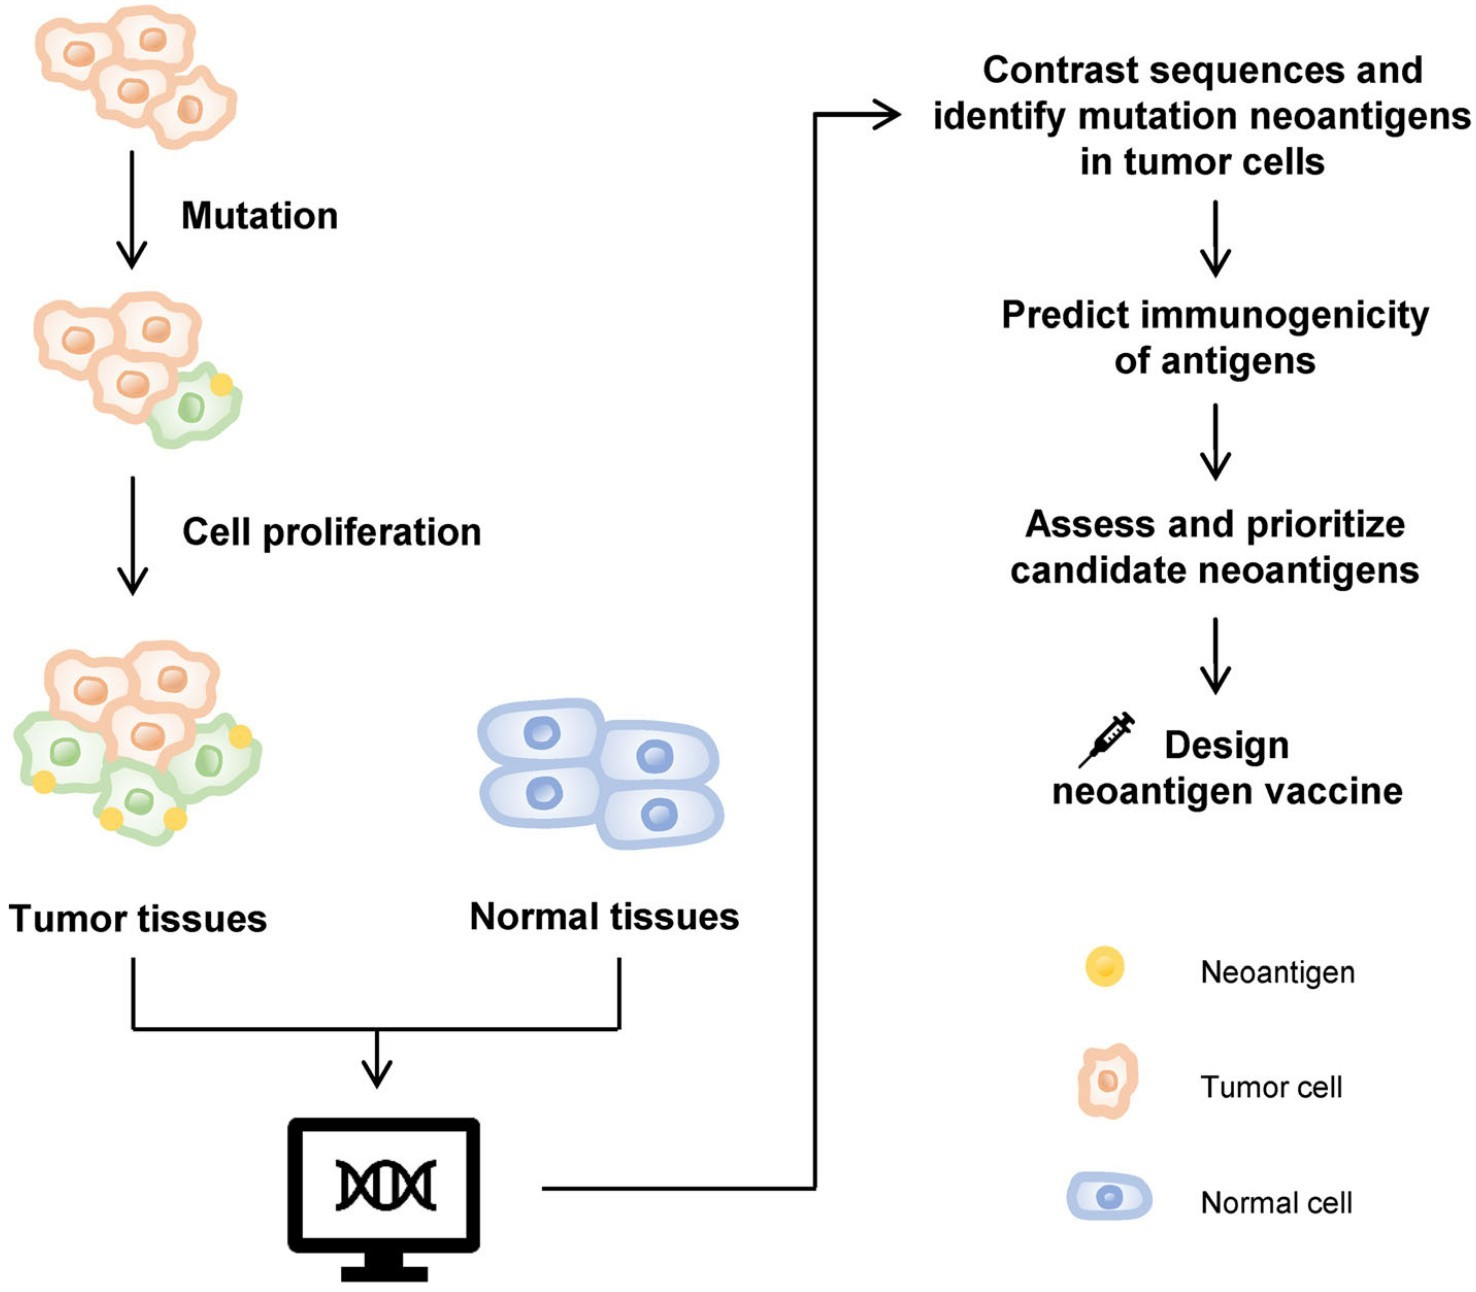
\includegraphics[width=0.6\textwidth]{img/neoantigen/process}
		\caption{Personalized vaccines process for Cancer \cite{peng2019neoantigen}.}
	\end{figure}		
\end{frame}
%-------------------------------------------------------
%-------------------------------------------------------



%-------------------------------------------------------
%-------------------------------------------------------
\begin{frame}{pMHC binding and presentation prediction}{}		
	\begin{figure}[H]
		\centering
		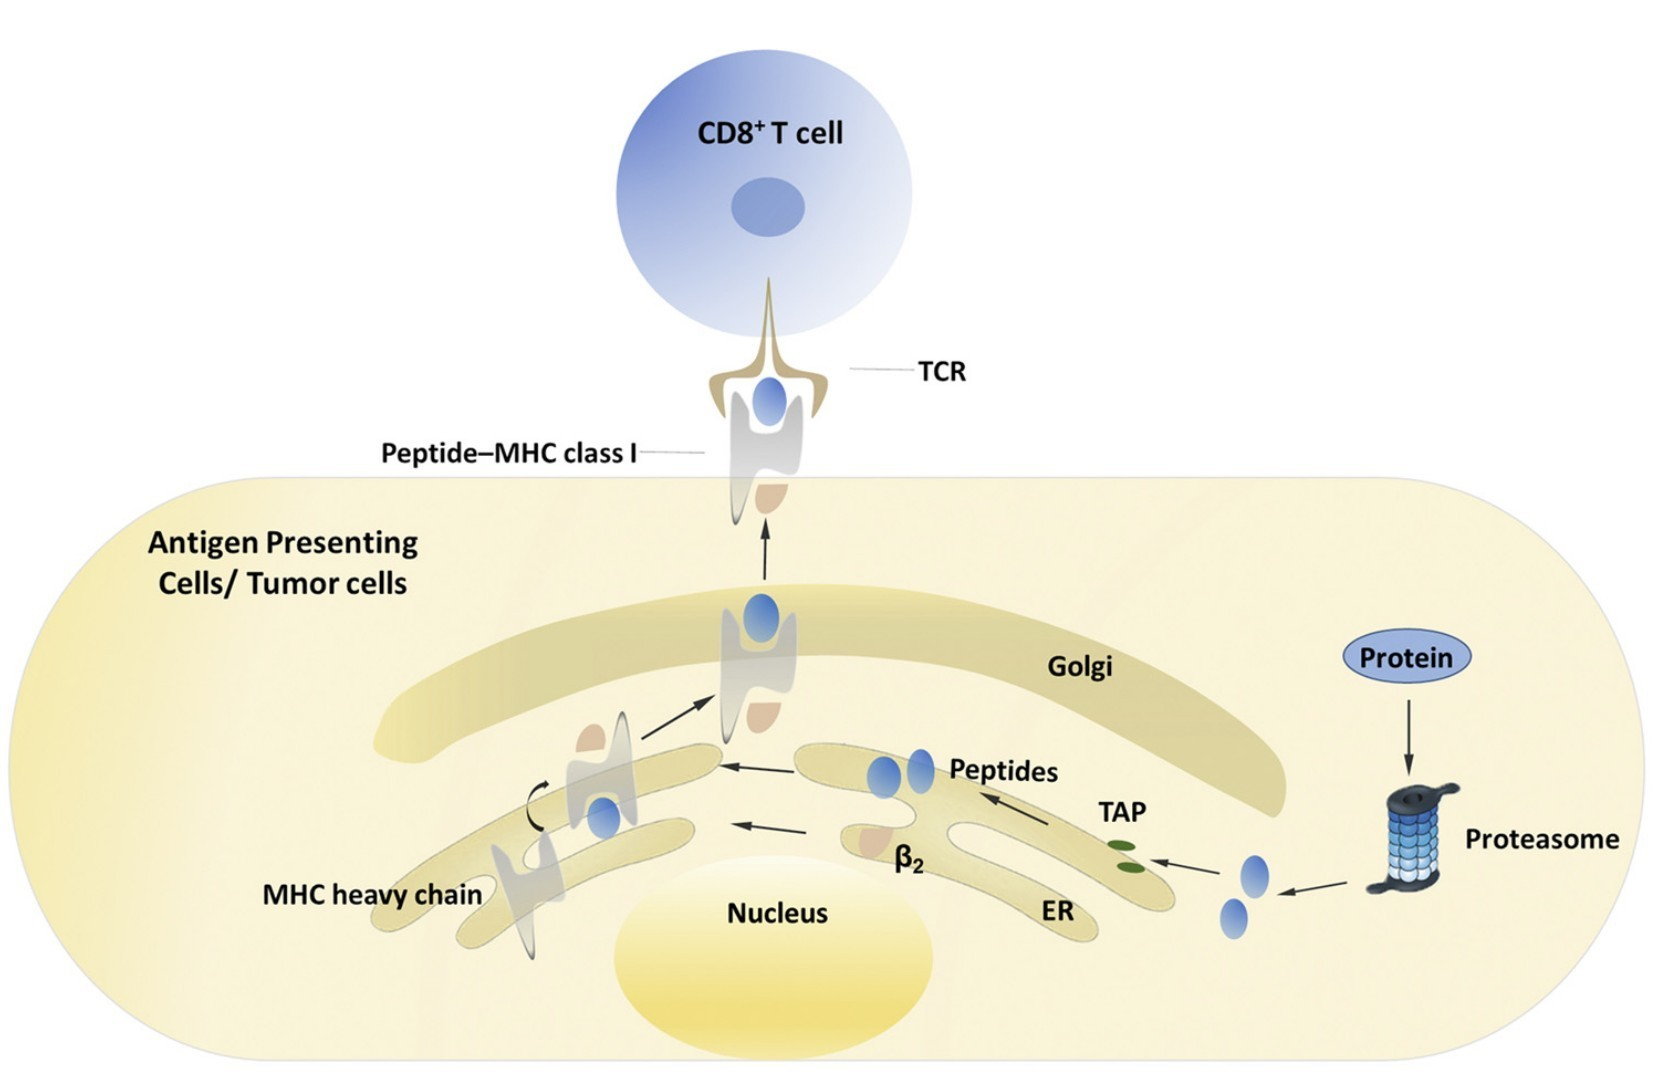
\includegraphics[width=0.9\textwidth]{img/neoantigen/mhc1.jpg}
		\caption{pMHC presentation process in MHC class I \cite{zhang2019application}.}
		\label{fig:mhc1}
	\end{figure}	
\end{frame}
%-------------------------------------------------------
%-------------------------------------------------------






%-------------------------------------------------------
%-------------------------------------------------------
%\begin{frame}{Objetivos}{}	
%	\begin{figure}
%		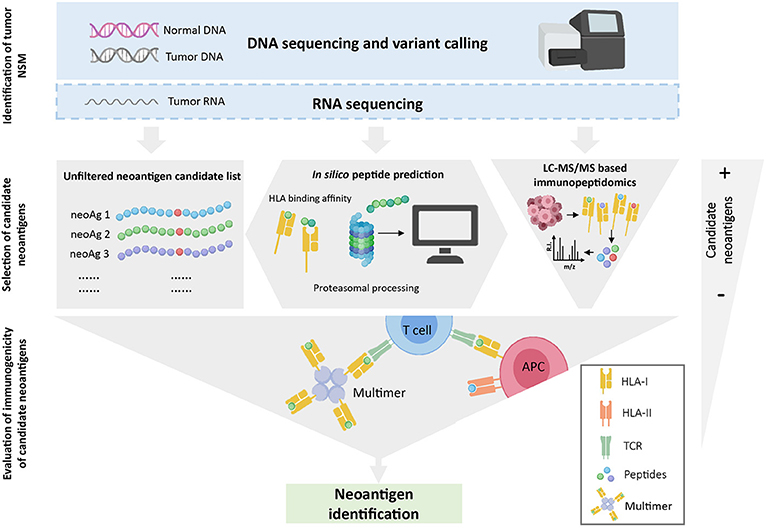
\includegraphics[width=0.97\textwidth]{img/neoantigen/pipeline_neoantigen}
		%\caption{Proceso de la detección de neo antígenos \cite{garcia2019determinants}.}
%	\end{figure}
%\end{frame}
%-------------------------------------------------------
%-------------------------------------------------------


%%%%%%%%%%%%%%%%%%%%%%%%%%%%%%%%%%%%%%%%%%%%%%%%%%%%%%%%%%%%%%%%%%%%%%%%%%%%%%%%%%%%%%%%%%%%%%%%%%%%%%%%%%%%%%%%
%%%%%%%%%%%%%%%%%%%%%%%%%%%%%%%%%%%%%%%%%%%%%%%%%%%%%%%%%%%%%%%%%%%%%%%%%%%%%%%%%%%%%%
\section{Methodology}
%%%%%%%%%%%%%%%%%%%%%%%%%%%%%%%%%%%%%%%%%%%%%%%%%%%%%%%%%%%%%%%%%%%%%%%%%%%%%%%%%%%%%%%%%%%%%%%%%%%%%%%%%%%%%%%%
%%%%%%%%%%%%%%%%%%%%%%%%%%%%%%%%%%%%%%%%%%%%%%%%%%%%%%%%%%%%%%%%%%%%%%%%%%%%%%%%%%%%%%

%%%%%%%%%%%%%%%%%%%%%%%%%%%%%%%%%%%%%%%%%%%%%%%%%%%%%%%%%%%%%%%%%%%%%%%%%%%%%%%%%%%%%%%%%%%%%%%%%%%%%%%%%%%%%%%%
%%%%%%%%%%%%%%%%%%%%%%%%%%%%%%%%%%%%%%%%%%%%%%%%%%%%%%%%%%%%%%%%%%%%%%%%%%%%%%%%%%%%%%
\subsection{Research Questions}
%%%%%%%%%%%%%%%%%%%%%%%%%%%%%%%%%%%%%%%%%%%%%%%%%%%%%%%%%%%%%%%%%%%%%%%%%%%%%%%%%%%%%%%%%%%%%%%%%%%%%%%%%%%%%%%%
%%%%%%%%%%%%%%%%%%%%%%%%%%%%%%%%%%%%%%%%%%%%%%%%%%%%%%%%%%%%%%%%%%%%%%%%%%%%%%%%%%%%%%

%-------------------------------------------------------
%-------------------------------------------------------
\begin{frame}{Research Questions}{}
		\begin{table}[h]
		\begin{center}
			\caption{Research questions used in SLR.}
			\label{tab:questions}
			\setlength{\tabcolsep}{0.5em} % for the horizontal padding
			{\renewcommand{\arraystretch}{1.4}% for the vertical padding
				\begin{tabular}{p{8.5cm}}
					\textbf{Research questions} \\ \hline
					\textbf{Q1}. How deep learning and transformers are used in MHC-peptide binding and presentation prediction? \\
					\textbf{Q2}. What type of input data and pre-processing methods are used? \\
					\textbf{Q3}. Which are the most promising methods? \\		
				\end{tabular}
			}
		\end{center}
	\end{table}	

\end{frame}
%-------------------------------------------------------
%-------------------------------------------------------

%%%%%%%%%%%%%%%%%%%%%%%%%%%%%%%%%%%%%%%%%%%%%%%%%%%%%%%%%%%%%%%%%%%%%%%%%%%%%%%%%%%%%%%%%%%%%%%%%%%%%%%%%%%%%%%%
%%%%%%%%%%%%%%%%%%%%%%%%%%%%%%%%%%%%%%%%%%%%%%%%%%%%%%%%%%%%%%%%%%%%%%%%%%%%%%%%%%%%%%
\subsection{Search Strings}
%%%%%%%%%%%%%%%%%%%%%%%%%%%%%%%%%%%%%%%%%%%%%%%%%%%%%%%%%%%%%%%%%%%%%%%%%%%%%%%%%%%%%%%%%%%%%%%%%%%%%%%%%%%%%%%%
%%%%%%%%%%%%%%%%%%%%%%%%%%%%%%%%%%%%%%%%%%%%%%%%%%%%%%%%%%%%%%%%%%%%%%%%%%%%%%%%%%%%%%


%-------------------------------------------------------
%-------------------------------------------------------
\begin{frame}{Search Strings}{}
	We searched in IEEE Xplore, Science Direct, Springer, ACM Digital Library, PubMed, and Scopus.	
	
	
	\begin{table}[H]
		\begin{center}
			\caption{Search string used in SLR.}
			\label{tab:key_words}
			\setlength{\tabcolsep}{0.5em} % for the horizontal padding
			{\renewcommand{\arraystretch}{1.4}% for the vertical padding
				\begin{tabular}{p{10cm}}
					\textbf{Search Strings} \\ \hline
					(MHC-I OR MHC-II OR MHC OR HLA) AND (peptide OR epitope) AND (binding OR affinity OR prediction OR detection OR presentation) OR (neoantigen detection)                                                                                                      \\		
				\end{tabular}
			}
		\end{center}
	\end{table}
\end{frame}
%-------------------------------------------------------
%-------------------------------------------------------

%%%%%%%%%%%%%%%%%%%%%%%%%%%%%%%%%%%%%%%%%%%%%%%%%%%%%%%%%%%%%%%%%%%%%%%%%%%%%%%%%%%%%%%%%%%%%%%%%%%%%%%%%%%%%%%%
%%%%%%%%%%%%%%%%%%%%%%%%%%%%%%%%%%%%%%%%%%%%%%%%%%%%%%%%%%%%%%%%%%%%%%%%%%%%%%%%%%%%%%
\subsection{Results}
%%%%%%%%%%%%%%%%%%%%%%%%%%%%%%%%%%%%%%%%%%%%%%%%%%%%%%%%%%%%%%%%%%%%%%%%%%%%%%%%%%%%%%%%%%%%%%%%%%%%%%%%%%%%%%%%
%%%%%%%%%%%%%%%%%%%%%%%%%%%%%%%%%%%%%%%%%%%%%%%%%%%%%%%%%%%%%%%%%%%%%%%%%%%%%%%%%%%%%%


%-------------------------------------------------------
%-------------------------------------------------------
\begin{frame}{Inclusion Criteria}{}
	
	\begin{block}{}
		Conference papers with ERA category (A or B) or journal articles Q1/Q2. Moreover, papers published since 2018.
	\end{block}
	
\end{frame}
%-------------------------------------------------------
%-------------------------------------------------------

%-------------------------------------------------------
%-------------------------------------------------------
\begin{frame}{Results}{}

We analyzed papers' titles, and then  a small subset of \textbf{54 papers were selected}.

	\begin{table}[H]
		\begin{center}
			\caption{Number of papers found in databases according to search string. }
			\label{tab:number_papers}
			\setlength{\tabcolsep}{0.5em} % for the horizontal padding
			{\renewcommand{\arraystretch}{1.2}% for the vertical padding
				\begin{tabular}{cc}
					\textbf{Year} & \textbf{Research papers} \\ \hline
					2018 & 46  \\
					2019 & 72  \\
					2020 & 86  \\
					2021 & 61  \\
					2022 & 58  \\ \hline
					Total & \textbf{323} \\
				\end{tabular}
			}
		\end{center}
	\end{table}
	
\end{frame}
%-------------------------------------------------------
%-------------------------------------------------------


%%%%%%%%%%%%%%%%%%%%%%%%%%%%%%%%%%%%%%%%%%%%%%%%%%%%%%%%%%%%%%%%%%%%%%%%%%%%%%%%%%%%%%%%%%%%%%%%%%%%%%%%%%%%%%%%
%%%%%%%%%%%%%%%%%%%%%%%%%%%%%%%%%%%%%%%%%%%%%%%%%%%%%%%%%%%%%%%%%%%%%%%%%%%%%%%%%%%%%%
\section{Input Encoding}
%%%%%%%%%%%%%%%%%%%%%%%%%%%%%%%%%%%%%%%%%%%%%%%%%%%%%%%%%%%%%%%%%%%%%%%%%%%%%%%%%%%%%%%%%%%%%%%%%%%%%%%%%%%%%%%%
%%%%%%%%%%%%%%%%%%%%%%%%%%%%%%%%%%%%%%%%%%%%%%%%%%%%%%%%%%%%%%%%%%%%%%%%%%%%%%%%%%%%%%


%%%%%%%%%%%%%%%%%%%%%%%%%%%%%%%%%%%%%%%%%%%%%%%%%%%%%%%%%%%%%%%%%%%%%%%%%%%%%%%%%%%%%%%%%%%%%%%%%%%%%%%%%%%%%%%%
%%%%%%%%%%%%%%%%%%%%%%%%%%%%%%%%%%%%%%%%%%%%%%%%%%%%%%%%%%%%%%%%%%%%%%%%%%%%%%%%%%%%%%
\subsection{Input Encoding}
%%%%%%%%%%%%%%%%%%%%%%%%%%%%%%%%%%%%%%%%%%%%%%%%%%%%%%%%%%%%%%%%%%%%%%%%%%%%%%%%%%%%%%%%%%%%%%%%%%%%%%%%%%%%%%%%
%%%%%%%%%%%%%%%%%%%%%%%%%%%%%%%%%%%%%%%%%%%%%%%%%%%%%%%%%%%%%%%%%%%%%%%%%%%%%%%%%%%%%%

%-------------------------------------------------------
%-------------------------------------------------------
\begin{frame}{Input Encoding}{}
	\begin{block}{}
		This is a \textbf{binary classification problem}. A peptide could be represented like: $p = \{ A, ... , Q \}$ and a MHC like: $q = \{ A, N, ... ,Q, E \}$. Finally, we need to know the probability of affinity between $p$ and $q$ (pMHC)
	\end{block}

\end{frame}
%-------------------------------------------------------
%-------------------------------------------------------

%-------------------------------------------------------
%-------------------------------------------------------
\begin{frame}{Input Encoding}{One-hot}	
	
	\begin{figure}[H]
		\centering
		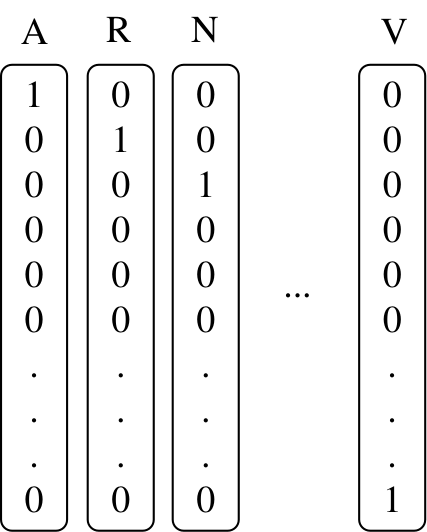
\includegraphics[width=0.3\textwidth]{img/neoantigen/onehot}
		\caption{pMHC presentation process in MHC class I \cite{zhang2019application}.}		
	\end{figure}
\end{frame}
%-------------------------------------------------------
%-------------------------------------------------------


%-------------------------------------------------------
%-------------------------------------------------------
\begin{frame}{Input Encoding}{BLOSUM}	
	\begin{table}[]
		\tiny
		\centering
		\caption{BLOSUM62 matrix. Normally, it is used to represent amino acids numerically. Each amino acid is represented by a row.}
		\label{tab:blosum62}
		\setlength{\tabcolsep}{0.5em} % for the horizontal padding
		{\renewcommand{\arraystretch}{1.2}% for the vertical padding
			
			
			\begin{tabular}{lllllllllllllllllllll}
				& \textbf{C} & \textbf{S} & \textbf{T} & \textbf{P} & \textbf{A} & \textbf{G} & \textbf{N} & \textbf{D} & \textbf{E} & \textbf{Q} & \textbf{H} & \textbf{R} & \textbf{K} & \textbf{M} & \textbf{I} & \textbf{L} & \textbf{V} & \textbf{F} & \textbf{Y} & \textbf{W} \\
				\textbf{C} & 0          &            &            &            &            &            &            &            &            &            &            &            &            &            &            &            &            &            &            &            \\
				\textbf{S} & -1         & 4          &            &            &            &            &            &            &            &            &            &            &            &            &            &            &            &            &            &            \\
				\textbf{T} & -1         & 1          & 5          &            &            &            &            &            &            &            &            &            &            &            &            &            &            &            &            &            \\
				\textbf{P} & -3         & -1         & -1         & 7          &            &            &            &            &            &            &            &            &            &            &            &            &            &            &            &            \\
				\textbf{A} & 0          & 1          & 0          & -1         & 4          &            &            &            &            &            &            &            &            &            &            &            &            &            &            &            \\
				\textbf{G} & -3         & 0          & -2         & -2         & 0          & 6          &            &            &            &            &            &            &            &            &            &            &            &            &            &            \\
				\textbf{N} & -3         & -1         & 0          & -2         & -2         & 0          & 6          &            &            &            &            &            &            &            &            &            &            &            &            &            \\
				\textbf{D} & -3         & 1          & -1         & -1         & -2         & -1         & 1          & 6          &            &            &            &            &            &            &            &            &            &            &            &            \\
				\textbf{E} & -4         & 0          & -1         & -1         & -1         & -2         & 0          & 2          & 5          &            &            &            &            &            &            &            &            &            &            &            \\
				\textbf{Q} & -3         & 0          & -1         & -1         & -1         & -2         & 0          & 0          & 2          & 5          &            &            &            &            &            &            &            &            &            &            \\
				\textbf{H} & -3         & 0          & -2         & -2         & -2         & -2         & 1          & -1         & 0          & 0          & 8          &            &            &            &            &            &            &            &            &            \\
				\textbf{R} & -3         & -1         & -1         & -2         & -1         & -2         & 0          & -2         & 0          & 1          & 0          & 5          &            &            &            &            &            &            &            &            \\
				\textbf{K} & -3         & -1         & -1         & -1         & -1         & -2         & 0          & -1         & 1          & 1          & -1         & 2          & 5          &            &            &            &            &            &            &            \\
				\textbf{M} & -1         & 0          & -1         & -2         & -1         & -3         & -2         & -3         & -2         & 0          & -2         & -1         & -1         & 5          &            &            &            &            &            &            \\
				\textbf{I} & -1         & -2         & -1         & -3         & -1         & -1         & -4         & -3         & -3         & -3         & -3         & -3         & -3         & 1          & 4          &            &            &            &            &            \\
				\textbf{L} & -1         & -2         & -1         & -3         & -1         & -4         & -3         & -4         & -3         & -2         & -3         & -2         & -2         & 2          & 2          & 4          &            &            &            &            \\
				\textbf{V} & -1         & -2         & 0          & -2         & 0          & -3         & -3         & -3         & -2         & -2         & -3         & -3         & -2         & 1          & 3          & 1          & 4          &            &            &            \\
				\textbf{F} & -2         & -2         & -2         & -4         & -2         & -3         & -3         & -3         & -3         & -3         & -1         & -3         & -3         & 0          & 0          & 0          & -1         & 6          &            &            \\
				\textbf{Y} & -2         & -2         & -2         & -3         & -2         & -3         & -2         & -3         & -2         & -1         & 2          & -2         & -2         & -1         & -1         & -1         & -1         & 3          & 7          &            \\
				\textbf{W} & -2         & -3         & -2         & -4         & -3         & -2         & -4         & -4         & -3         & -2         & -2         & -3         & -3         & -1-        & -3         & -2         & -3         & 1          & 2          & 11        
			\end{tabular}
			
		}
	\end{table}

\end{frame}
%-------------------------------------------------------
%-------------------------------------------------------


%-------------------------------------------------------
%-------------------------------------------------------
\begin{frame}{Input Encoding}{Another Alternatives}	
	
	\begin{block}{}
		Also, there are another alternatives like: universal \textbf{Google encoder} \cite{kubick2021predicting}, \textbf{AAindex} \cite{kawashima2000aaindex,li2021deepimmuno}  (a database  of numerical indices representing physicochemical and biochemical properties of amino acids), \textbf{3D amino acid coordinates} \cite{shi2020deepantigen}, and \textbf{physicochemical properties} of each amino acid \cite{moris2021current,montemurro2021nettcr,luu2021predicting}. 
	\end{block}
\end{frame}
%-------------------------------------------------------
%-------------------------------------------------------



%%%%%%%%%%%%%%%%%%%%%%%%%%%%%%%%%%%%%%%%%%%%%%%%%%%%%%%%%%%%%%%%%%%%%%%%%%%%%%%%%%%%%%%%%%%%%%%%%%%%%%%%%%%%%%%%
%%%%%%%%%%%%%%%%%%%%%%%%%%%%%%%%%%%%%%%%%%%%%%%%%%%%%%%%%%%%%%%%%%%%%%%%%%%%%%%%%%%%%%
\section{How Deep Learning is used?}
%%%%%%%%%%%%%%%%%%%%%%%%%%%%%%%%%%%%%%%%%%%%%%%%%%%%%%%%%%%%%%%%%%%%%%%%%%%%%%%%%%%%%%%%%%%%%%%%%%%%%%%%%%%%%%%%
%%%%%%%%%%%%%%%%%%%%%%%%%%%%%%%%%%%%%%%%%%%%%%%%%%%%%%%%%%%%%%%%%%%%%%%%%%%%%%%%%%%%%%


%%%%%%%%%%%%%%%%%%%%%%%%%%%%%%%%%%%%%%%%%%%%%%%%%%%%%%%%%%%%%%%%%%%%%%%%%%%%%%%%%%%%%%%%%%%%%%%%%%%%%%%%%%%%%%%%
%%%%%%%%%%%%%%%%%%%%%%%%%%%%%%%%%%%%%%%%%%%%%%%%%%%%%%%%%%%%%%%%%%%%%%%%%%%%%%%%%%%%%%
\subsection{DANN, CNN, and RNN }
%%%%%%%%%%%%%%%%%%%%%%%%%%%%%%%%%%%%%%%%%%%%%%%%%%%%%%%%%%%%%%%%%%%%%%%%%%%%%%%%%%%%%%%%%%%%%%%%%%%%%%%%%%%%%%%%
%%%%%%%%%%%%%%%%%%%%%%%%%%%%%%%%%%%%%%%%%%%%%%%%%%%%%%%%%%%%%%%%%%%%%%%%%%%%%%%%%%%%%%


%-------------------------------------------------------
%-------------------------------------------------------
\begin{frame}{DANN, CNN, and RNN }{}
		
	\begin{block}{}
		Currently, the state-of-art method is \textbf{NetMHCPan4.1} \cite{reynisson2020netmhcpan}, it is a DANN of 40 assembled ANNs with 60 and 70 neurons. Additionally, it uses NN\_alignMA \cite{alvarez2019nnalign_ma} to handle poly-specific datasets of Mass Spectrometry (MS)-eluted ligands. 
	\end{block}	
	
\end{frame}
%-------------------------------------------------------
%-------------------------------------------------------


%-------------------------------------------------------
%-------------------------------------------------------
\begin{frame}{DANN, CNN, and RNN }{Convolutional Neural Networks}
	
	\fontsize{8pt}{5pt}\selectfont
	
	\begin{table}[]
		\centering
		\caption{List of research since 2018 that uses CNNs for peptide-MHC binding and presentation.}
		\setlength{\tabcolsep}{0.5em} % for the horizontal padding
		{\renewcommand{\arraystretch}{2}% for the vertical padding
			\begin{tabular}{p{0.6cm}p{0.6cm}p{1.5cm}p{2cm}p{0.6cm}p{2.7cm}}
				\textbf{Year} & \textbf{Ref.}                              & \textbf{Approach}        & \textbf{Name} & \textbf{MHC} & \textbf{Encoding}                                                                                                                                                                                   \\ \hline
				
				2022 &	\cite{you2022deepmhcii}	& pMHC(b) &	DeepMHCII &	 II &	PFR \\
				
				2021          & \cite{li2021deepimmuno}   & pMHC(b)      & DeepImmuno    &  I        & AAindex1                                                \\
				2021          & \cite{lang2021neofox}     & pMHC(p) & APPM          &  I        & One-hot                                                                          \\
				2021          & \cite{lee2021connecting}  & pMHC(p) & MHCfovea      &  I        & One-hot                                                                                                      \\
				2021          & \cite{junet2021cnn}       & pMHC(b)      & CNN-PepPred   &  II       & BLOSUM     \\
				
				2020          & \cite{pei2020iconmhc}     & pMHC(b)      & IConMHC       & I        & PCA and AAindex3        \\
				2020          & \cite{saxena2020onionmhc} & pMHC(b)      & OnionMHC      & I        & BLOSUM and structural features                                                                  \\
				2020          & \cite{ng3704016minerva}   & pMHC(p) & MINERVA       & I        & Physicochemical properties                                                           \\
				2019          & \cite{zhao2019peptide}    & pMHC(b)      & CNN-NF        & I        & Sequence, Hydropathy, Polarity, Length                    \\
				2019          & \cite{liu2019deepseqpan}  & pMHC(b)      & DeepSeqPan    & I        & One-hot                                          \\
				2018          & \cite{han2018deep}        & pMHC(b)      & ConvMHC       & I        & Contact side HLA.peptide                                                                                 
			\end{tabular}
		}
	\end{table}	
\end{frame}
%-------------------------------------------------------
%-------------------------------------------------------

%-------------------------------------------------------
%-------------------------------------------------------
\begin{frame}{DANN, CNN, and RNN }{Recurrent Neural Networks}
	
	\fontsize{8pt}{5pt}\selectfont
	
	\begin{table}[]
		\centering
		\caption{List of research since 2018 that uses RNNs for peptide-MHC binding and presentation. MATHLA, DeepSeqPanII and DeepHLApan uses RNN with attention mechanims, meanwhile the other focus on GRU and LSTM.}		
		\setlength{\tabcolsep}{0.5em} % for the horizontal padding
		{\renewcommand{\arraystretch}{2}% for the vertical padding
			\begin{tabular}{p{0.6cm}p{0.6cm}p{1.5cm}p{2cm}p{0.6cm}p{2.7cm}}
				\textbf{Year} & \textbf{Ref.}                               & \textbf{Approach}   & \textbf{Name} & \textbf{MHC} & \textbf{Encoding}                                                                                                                                                                                                                         \\ \hline
				2021          & \cite{ye2021mathla}        & pMHC(b) & MATHLA        & I        & BLOSUM                      \\
				
				2021          & \cite{liu2021deepseqpanii} & pMHC(b)                     & DeepSeqPanII                      & II       & One-hot  and BLOSUM                                                    \\
				
				2021          & \cite{heng2021simple}      & pMHC(b)                     & GRU-based RNN                     & II       & Embeding layer                                                        \\
				
				2021          & \cite{jiang2021predicting} & pMHC(b)                     & BVLSTM-MHC                        & I        & One-hot  and BLOSUM                                                                        \\
				
				2020          & \cite{shao2020high}        & pMHC(b)                     & MHCnuggets                        & I, II & One-hot                \\
				
				2019          & \cite{wu2019deephlapan}    & pMHC(b)                     & DeepHLApan                        & I        & One-hot                     
			\end{tabular}
		}
	\end{table}	
\end{frame}
%-------------------------------------------------------
%-------------------------------------------------------

%%%%%%%%%%%%%%%%%%%%%%%%%%%%%%%%%%%%%%%%%%%%%%%%%%%%%%%%%%%%%%%%%%%%%%%%%%%%%%%%%%%%%%%%%%%%%%%%%%%%%%%%%%%%%%%%
%%%%%%%%%%%%%%%%%%%%%%%%%%%%%%%%%%%%%%%%%%%%%%%%%%%%%%%%%%%%%%%%%%%%%%%%%%%%%%%%%%%%%%
\subsection{ Transformers }
%%%%%%%%%%%%%%%%%%%%%%%%%%%%%%%%%%%%%%%%%%%%%%%%%%%%%%%%%%%%%%%%%%%%%%%%%%%%%%%%%%%%%%%%%%%%%%%%%%%%%%%%%%%%%%%%
%%%%%%%%%%%%%%%%%%%%%%%%%%%%%%%%%%%%%%%%%%%%%%%%%%%%%%%%%%%%%%%%%%%%%%%%%%%%%%%%%%%%%%



%-------------------------------------------------------
%-------------------------------------------------------
\begin{frame}{Transformers}{}
	
	\begin{block}{}
		The \textbf{Transformer Neural Network} is a novel architecture that aims to solve sequence-to-sequence tasks while handling long-range dependencies with ease. It was proposed in the paper ``Attention Is All You Need'' \cite{vaswani2017attention}. 
	\end{block}

	\begin{block}{}
		\textbf{Bidirectional Encoder Representations from Transformers (BERT)} \cite{devlin2018bert} is a recent paper published by researchers at Google AI Language. It has caused a stir in the Machine Learning community by presenting state-of-the-art results in a wide variety of NLP tasks,
	\end{block}
	
\end{frame}
%-------------------------------------------------------
%-------------------------------------------------------


%-------------------------------------------------------
%-------------------------------------------------------
\begin{frame}{Transformers}{Transfer Learning}
	
	%\fontsize{12pt}{10pt}\selectfont
	\begin{table}[]
		
		\caption{List of pre-trained BERT models.}
		\setlength{\tabcolsep}{0.8em} % for the horizontal padding
		{\renewcommand{\arraystretch}{1.1}% for the vertical padding
			
		\begin{tabular}{lp{3cm}p{3cm}}
			\textbf{Model} & \textbf{Parameters}          & \textbf{Layers} \\ \hline
			TAPE           & 92M                          & 12                        \\
			ProtBert       & 420M                         & 30                        \\
			ESM1           & 43M, 85M y 670M              & 6, 12, and 34             \\
			ESM1-b         & 650M                         & 33                        \\
			ESM2           & 8M, 35M, 150M, 650M, 3B, 15B & 6, 12, 30, 33, 36, and 48
		\end{tabular}
	
	}
	\end{table}
	
	
\end{frame}
%-------------------------------------------------------
%-------------------------------------------------------


%-------------------------------------------------------
%-------------------------------------------------------
\begin{frame}{Transformers}{}
	
	%\fontsize{12pt}{10pt}\selectfont
	
	 \begin{table}[]
	 	\caption{Transformers used for pMHC binding and presentation prediction.}
	 	\label{tab:transformes}
	 	\setlength{\tabcolsep}{0.5em} % for the horizontal padding
	 	{\renewcommand{\arraystretch}{1.1}% for the vertical padding
	 		
	 		\begin{footnotesize}
	 			\begin{tabular}{p{0.8cm}p{1.5cm}p{7.3cm}}
	 				\multicolumn{1}{l}{\textbf{Year}}                                   & \textbf{Name}                       & \textbf{Model}     \\  \hline
	 				
	 				2022\cite{zhang2022hlab}&	\textbf{HLAB}&	BERT from ProtBert pre-trained model followed by a BiLSTM with attention mechanism.	\\
	 				
	 				2022\cite{wang2022mhcroberta}          & MHC RoBERTa             &  RoBERTa  pre-trained and followed by 12 multi-head SA and a FC layers, it outperformed NetMHCPan 3.0.                                                                                          \\
	 				2022\cite{chu2022transformer}          & \textbf{TransPHLA}                     & It used SA mechanism based on four blocks, it slightly outperformed NetMHCpan4.1 and is faster making predictions.\\
	 				
	 				2021\cite{gasser2021interpreting}  & ImmunoBERT                              & BERT from TAPE pre-trained followed by a linear layer. Authors claimed that N-terminal and C-terminals are highly relevant after analysis with SHAP and LIME.   \\
	 				
	 				2021\cite{cheng2021bertmhc}             & BERTMHC                            & BERT from TAPE pre-trained followed by a linear layer. It outperformed NetMHCIIpan3.2 and PUFFIN.   \\
	 			                  
	 			\end{tabular}
	 		\end{footnotesize}
	 	}
	 \end{table}
	 
	 
\end{frame}
%-------------------------------------------------------
%-------------------------------------------------------






%%%%%%%%%%%%%%%%%%%%%%%%%%%%%%%%%%%%%%%%%%%%%%%%%%%%%%%%%%%%%%%%%%%%%%%%%%%%%%%%%%%%%%%%%%%%%%%%%%%%%%%%%%%%%%%%
%%%%%%%%%%%%%%%%%%%%%%%%%%%%%%%%%%%%%%%%%%%%%%%%%%%%%%%%%%%%%%%%%%%%%%%%%%%%%%%%%%%%%%
\section{ Which are the most promising methods?}
%%%%%%%%%%%%%%%%%%%%%%%%%%%%%%%%%%%%%%%%%%%%%%%%%%%%%%%%%%%%%%%%%%%%%%%%%%%%%%%%%%%%%%%%%%%%%%%%%%%%%%%%%%%%%%%%
%%%%%%%%%%%%%%%%%%%%%%%%%%%%%%%%%%%%%%%%%%%%%%%%%%%%%%%%%%%%%%%%%%%%%%%%%%%%%%%%%%%%%%

%%%%%%%%%%%%%%%%%%%%%%%%%%%%%%%%%%%%%%%%%%%%%%%%%%%%%%%%%%%%%%%%%%%%%%%%%%%%%%%%%%%%%%%%%%%%%%%%%%%%%%%%%%%%%%%%
%%%%%%%%%%%%%%%%%%%%%%%%%%%%%%%%%%%%%%%%%%%%%%%%%%%%%%%%%%%%%%%%%%%%%%%%%%%%%%%%%%%%%%
\subsection{ State-of-art methods}
%%%%%%%%%%%%%%%%%%%%%%%%%%%%%%%%%%%%%%%%%%%%%%%%%%%%%%%%%%%%%%%%%%%%%%%%%%%%%%%%%%%%%%%%%%%%%%%%%%%%%%%%%%%%%%%%
%%%%%%%%%%%%%%%%%%%%%%%%%%%%%%%%%%%%%%%%%%%%%%%%%%%%%%%%%%%%%%%%%%%%%%%%%%%%%%%%%%%%%%

%-------------------------------------------------------
%-------------------------------------------------------
\begin{frame}{State of art methods}{}
	
	\begin{block}{}
		Although \textbf{NetMHCpan4.1} is the state-of-art pan method, the transformers overcome exciting results. These BERT models \cite{cheng2021bertmhc,gasser2021interpreting,wang2022mhcroberta}, used transfer learning from TAPE \cite{rao2019evaluating}, and ProtBert \cite{elnaggar2021prottrans}, which are models self-supervised trained with Pfam, UniRef50, UniRef100, UniProtKB, Swiss-prot and BFD datasets. 
	\end{block}
	
	\begin{block}{}
		Despite, NetMHCpan4.1 \cite{reynisson2020netmhcpan} is considered the state-of-the-art pan-specific method; \textbf{HLAB}  \cite{zhang2022hlab} and \textbf{TransPHLA} \cite{chu2022transformer}  slightly outperformed it on allele-specific testing. 
	\end{block}
	
\end{frame}
%-------------------------------------------------------
%-------------------------------------------------------

%%%%%%%%%%%%%%%%%%%%%%%%%%%%%%%%%%%%%%%%%%%%%%%%%%%%%%%%%%%%%%%%%%%%%%%%%%%%%%%%%%%%%%%%%%%%%%%%%%%%%%%%%%%%%%%%
%%%%%%%%%%%%%%%%%%%%%%%%%%%%%%%%%%%%%%%%%%%%%%%%%%%%%%%%%%%%%%%%%%%%%%%%%%%%%%%%%%%%%%
\subsection{ Limitations }
%%%%%%%%%%%%%%%%%%%%%%%%%%%%%%%%%%%%%%%%%%%%%%%%%%%%%%%%%%%%%%%%%%%%%%%%%%%%%%%%%%%%%%%%%%%%%%%%%%%%%%%%%%%%%%%%
%%%%%%%%%%%%%%%%%%%%%%%%%%%%%%%%%%%%%%%%%%%%%%%%%%%%%%%%%%%%%%%%%%%%%%%%%%%%%%%%%%%%%%

%-------------------------------------------------------
%-------------------------------------------------------
\begin{frame}{Limitations}{}
	
	\begin{block}{}
		They ignored Posttranslational modifications (PTMs) such as phosphorylation, glycosylation, and deamidation, which influence the specificity of MHC binding and presentation and several aspects of the biology underlying pMHC presentation are poorly understood. Furthermore, to get accurate results for neoantigen detection, we need to integrate pMHC-TCR studies. 
	\end{block}

	\begin{block}{}
		Another limitations are related to high computing requirements for training BERT architectures. For instance, the biggest ESM2 model has 15 billion parameters.
	\end{block}

\end{frame}
%-------------------------------------------------------
%-------------------------------------------------------

%%%%%%%%%%%%%%%%%%%%%%%%%%%%%%%%%%%%%%%%%%%%%%%%%%%%%%%%%%%%%%%%%%%%%%%%%%%%%%%%%%%%%%%%%%%%%%%%%%%%%%%%%%%%%%%%
%%%%%%%%%%%%%%%%%%%%%%%%%%%%%%%%%%%%%%%%%%%%%%%%%%%%%%%%%%%%%%%%%%%%%%%%%%%%%%%%%%%%%%
\subsection{ Future works }
%%%%%%%%%%%%%%%%%%%%%%%%%%%%%%%%%%%%%%%%%%%%%%%%%%%%%%%%%%%%%%%%%%%%%%%%%%%%%%%%%%%%%%%%%%%%%%%%%%%%%%%%%%%%%%%%
%%%%%%%%%%%%%%%%%%%%%%%%%%%%%%%%%%%%%%%%%%%%%%%%%%%%%%%%%%%%%%%%%%%%%%%%%%%%%%%%%%%%%%

%-------------------------------------------------------
%-------------------------------------------------------
\begin{frame}{Future works}{}
	
	\begin{block}{}
		Future work could include the use of transfer learning from ESM1-b \cite{rives2021biological} and ESM2 \cite{lin2023evolutionary}. 
	\end{block}
	
	\begin{block}{}
		Moreover, there is pHLA3D, a dataset of 3D structures of the alpha/beta chains and peptides of MHC-I proteins; it opens new perspectives for studying pMHC prediction. 
	\end{block}
	
\end{frame}
%-------------------------------------------------------
%-------------------------------------------------------

%-------------------------------------------------------
%-------------------------------------------------------
\begin{frame}[allowframebreaks]
	\frametitle{References}
	%\bibliographystyle{amsalpha}
	\bibliographystyle{IEEEtran}
	\bibliography{Bibliography.bib}
\end{frame}
%-------------------------------------------------------
%-------------------------------------------------------

%-------------------------------------------------------
%-------------------------------------------------------
\if\mycmd1 % MY THEME
\1{
	{\1
		\begin{frame}[plain,noframenumbering]
			%\finalpage{Thank you}
			\begin{figure}[]
				\centering
				
\includegraphics[width=\textwidth,height=0.7\textheight,keepaspectratio]{img/question.png}
				%\label{img:mot2}
				%\caption{Image example in 2 gray levels.}
			\end{figure}
	\end{frame}}
	\else % CS THEME
	\begin{frame}{Questions?}
		\begin{figure}[]
			\centering
			
\includegraphics[width=\textwidth,height=0.7\textheight,keepaspectratio]{img/question.png}
			%\label{img:mot2}
			%\caption{Image example in 2 gray levels.}
		\end{figure}
		
	\end{frame}
	\fi
	%-------------------------------------------------------
	%-------------------------------------------------------
	

\end{document}